\documentclass{article}
\usepackage{listofitems}
\usepackage{etoolbox}
\usepackage{pgf}
\usepackage{xstring}
\usepackage{intcalc}

\usepackage{listings}

\newcommand{\operation}[1]{%
    \StrLeft{#1}{1}[\firstletter]%
    \ifdefstring{\firstletter}{n}
    {
        \pgfmathsetmacro{\cycle}{\fpeval{1+\cycle}}
        \evalCycle{\cycle}
    }
    {
        \pgfmathsetmacro{\cycle}{\fpeval{1+\cycle}}
        \evalCycle{\cycle}
        \pgfmathsetmacro{\cycle}{\fpeval{1+\cycle}}
        \evalCycle{\cycle}
    }

    \pgfmathsetmacro{\H}{\fpeval{\cycle-1}}
    \pgfmathsetmacro{\h}{\intcalcMod{\H}{40}}
    \pgfmathsetmacro{\s}{\fpeval{\screenIndex-1}}
    \pgfmathsetmacro{\S}{\fpeval{\screenIndex+1}}

    \ifnum\h=\s%
        %X
    \else
        \ifnum\h=\screenIndex%
            %X
        \else
            \ifnum\h=\S%
               %X
            \else
                %.
            \fi
        \fi
    \fi

    \ifnum\intcalcMod{\screenIndex}{40}=0
        \pgfmathsetmacro{\screenIndex}{1}
    \fi

    \pgfmathsetmacro{\screenIndex}{\fpeval{\screenIndex+1}}
}

\newcommand{\setNumber}[1]{%
    \pgfmathsetmacro{\nr}{#1}
}

\newcommand{\evalCycle}[1]{%
    \pgfmathsetmacro{\p}{#1}
    \ifnum\p=20%
        \pgfmathsetmacro{\signalStrength}{\fpeval{20*\points}}
        \pgfmathsetmacro{\sum}{\fpeval{\sum+\signalStrength}} 
    \fi%
    \ifnum\p=60%
        \pgfmathsetmacro{\signalStrength}{\fpeval{60*\points}}
        \pgfmathsetmacro{\sum}{\fpeval{\sum+\signalStrength}} 
    \fi%
    \ifnum\p=100%
        \pgfmathsetmacro{\signalStrength}{\fpeval{100*\points}}
        \pgfmathsetmacro{\sum}{\fpeval{\sum+\signalStrength}} 
    \fi%
    \ifnum\p=140%
        \pgfmathsetmacro{\signalStrength}{\fpeval{140*\points}}
        \pgfmathsetmacro{\sum}{\fpeval{\sum+\signalStrength}} 
    \fi%
    \ifnum\p=180%
        \pgfmathsetmacro{\signalStrength}{\fpeval{180*\points}}
        \pgfmathsetmacro{\sum}{\fpeval{\sum+\signalStrength}} 
    \fi%
    \ifnum\p=220%
        \pgfmathsetmacro{\signalStrength}{\fpeval{220*\points}}
        \pgfmathsetmacro{\sum}{\fpeval{\sum+\signalStrength}} 
    \fi%
}

\newcounter{cnt}

\begin{document}

\pgfmathsetmacro{\screenIndex}{1}
\pgfmathsetmacro{\points}{1}

\pgfmathsetmacro{\points}{1}
\pgfmathsetmacro{\cycle}{0}
\pgfmathsetmacro{\sum}{0}
\pgfmathsetmacro{\signalStrength}{0}

    \newread\file
    \openin\file=input.txt

    \loop\unless\ifeof\file%
        \read\file to\input%
        \setsepchar{ }%
        \readlist*\foo{\input}%
        \setcounter{cnt}{1}%
        \foreachitem\z\in\foo
        {%
            \ifnum\zcnt=1%
                \operation{\foo[\zcnt]}
            \fi%
            \ifnum\zcnt=2%
                \setNumber{\foo[\zcnt]}
                \pgfmathsetmacro{\points}{\fpeval{\nr+\points}}
            \fi%
        }%
    \repeat%


\section{Part1}

Solving such problems in \LaTeX sounds like a dump idea.
And this is totally true.
So it is possible to write something like code in \LaTeX but the real problem is that all you do is defining macros.
So it took me a while but I came up with a solution for Part 1.
Parsing input files is not that difficult.
The first problme that occured where nested loops.
Somehow if I am done with the inner one I also leave the outer one.
So some nice people on stackexchange had the same problem and the solution provided was what you can see in \ref{01}.\newline

\begin{lstlisting}[caption=nested loops, label=01, captionpos=b]
    \loop\unless\ifeof\file%
        \read\file to\input%
        \setsepchar{ }%
        \readlist*\foo{\input}%
        \setcounter{cnt}{1}%
        \foreachitem\z\in\foo
        {%
            \ifnum\zcnt=1%
                \operation{\foo[\zcnt]}
            \fi%
            \ifnum\zcnt=2%
                \setNumber{\foo[\zcnt]}
                \pgfmathsetmacro{\points}{\fpeval{\nr+\points}}
            \fi%
        }%
    \repeat%
\end{lstlisting}

As you can see the inner curly brackets solved that problem.
So you don't need them, or at least only need curly brackets around loop from time to time. 
It depends.

Afterwards I needed to calculate some stuff.
\LaTeX is also not made for doing this.
But luckily there are some packages like intcalc which are able to calculate.\newline
And putting all of it together I came up with the following number as solution for part 1: \sum 
And guess what after submitting \sum I saw the following:

\begin{figure}[h]
    \centering
    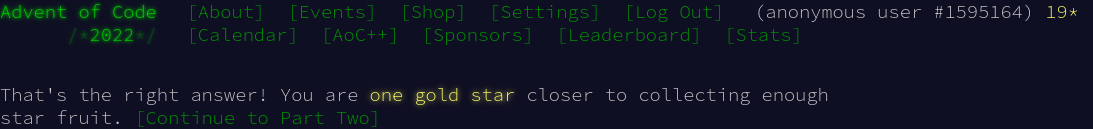
\includegraphics[width=1\textwidth]{ui.png}
    \caption{a nice plot}
    \label{02}
\end{figure}

So I onto part 2 I guess.

\section{Part 2}

Not so easy as I hoped.
Or at least not so easy to solve in \LaTeX.
The first problem and also the problem which leaded me to give up on this and do it in python was the following.
There is nothing like if a and b. 
And nothing like $a \leq b$.\newline
Well python also is a nice language.
And in compared to the \LaTeX stuff in about no time I came up with a solution.
All the magic behind are those 13 lines of code.

\begin{lstlisting}[caption=doing python, label=03, captionpos=b]
    def do_cycle():
    global crt
    global pixels

    if (cycle - 20) % 40 == 0:
        signal_strengths.append(cycle * X)

    pixels += "#" if X - 1 <= crt <= X + 1 else "."
    crt += 1 if crt < 39 else -39

    if crt == 0:
        pixels += "\n"

    return 1
\end{lstlisting}

Listing \ref{03} lead to the following.

\begin{lstlisting}[caption=help me to read, label=04, captionpos=b]
###..####.#..#.####..##..###..####.####.
#..#.#....#.#.....#.#..#.#..#.#....#....
#..#.###..##.....#..#....#..#.###..###..
###..#....#.#...#...#....###..#....#....
#.#..#....#.#..#....#..#.#....#....#....
#..#.#....#..#.####..##..#....####.#....
\end{lstlisting}

Idk it took me like 5 minutes to extract all the letters out of this stuff.

\end{document}